\chapter{Tutorial Blinky (Java)}

\section{Scope}

This tutorial describes how to use the \textit{TimingService}, how to combine a generated model with 
manual code and how to model a hierarchical state machine. The idea of the tutorial is to switch a LED on 
and off. The behavior of the LED should be: blinking in a one second interval for 5 seconds, stop blinking 
for 5 seconds, blinking, stop,...  
For this exercise we will use a little GUI class that will be used in more sophisticated tutorials too. 
The GUI simulates a pedestrian traffic crossing. For now, just a simple LED simulation will be used from 
the GUI. 

After the exercise is created you must copy the GUI to your src directory (see below).

The package contains four java classes which implements a small window with a 3-light traffic light which 
simulates the signals for the car traffic and a 2-light traffic light which simulates the pedestrian 
signals.

The GUI looks like this:

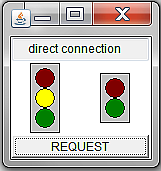
\includegraphics{images/020-Blinky08.png}
% !images/020-Blinky08.png!

Within this tutorial we will just toggle the yellow light.

You will perform the following steps:

\begin{enumerate}
\item create a new model from scratch
\item define a protocol
\item create an actor structure
\item create a hierarchical state machine
\item use the predefined \textit{TimingService}
\item combine manual code with generated code
\item build and run the model
\item open the message sequence chart
\end{enumerate}

\section{Create a new model from scratch}

Remember the exercise \textit{HelloWorld}.
Create a new \eTrice{} project and name it \textit{Blinky}.

To use the GUI please copy the package \textit{org.eclipse.etrice.tutorials.PedLightGUI} from 
\textit{org.eclipse.etrice.tutorials/src} to your \emph{src} directory \textit{Blinky/src}. For this tutorial 
you must remove the error markers by editing the file \textit{PedestrianLightWndNoTcp.java}. Appropriate 
comments are provided to remove the error markers for this turorial.

Open the \textit{Blinky.room} file and copy the following code into the file or use content assist to 
create the model.

\begin{verbatim} 
RoomModel Blinky {

    LogicalSystem System_Blinky {
        SubSystemRef subsystem : SubSystem_Blinky
    }

    SubSystemClass SubSystem_Blinky {
        ActorRef application : BlinkyTop
    }

    ActorClass BlinkyTop {
    }
}
\end{verbatim}

\section{Add two additional actor classes}

Position the cursor outside any class definition and right click the mouse within the editor window. From 
the context menu select \textit{Content Assist}  

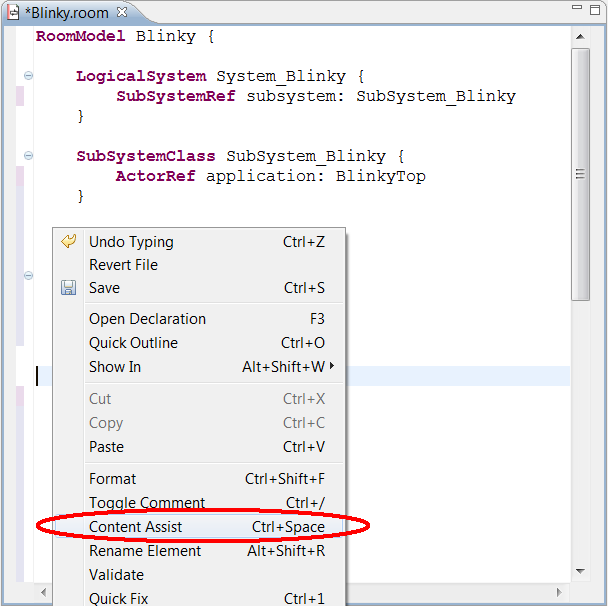
\includegraphics[width=0.8\textwidth]{images/020-Blinky02.png}
% !images/020-Blinky02.png!

Select \textit{ActorClass - actor class skeleton} and name it \textit{Blinky}.

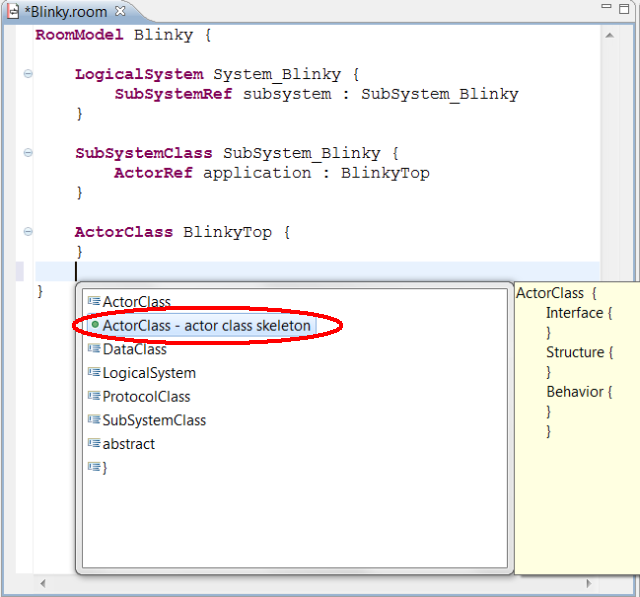
\includegraphics[width=0.8\textwidth]{images/020-Blinky01.png}
% !images/020-Blinky01.png! 

Repeat the described procedure and name the new actor \textit{BlinkyController}.

With Ctrl+Shift+F you can beautify the model code. 

Save the model and visit the outline view.

\section{Create a new protocol}

With the help of \textit{Content Assist} create a \textit{ProtocolClass} and name it 
\textit{BlinkyControlProtocol}.
Inside the brackets use the \textit{Content Assist} (CTRL+Space) to create two incoming messages called 
\textit{start} and \textit{stop}.

The resulting code should look like this:

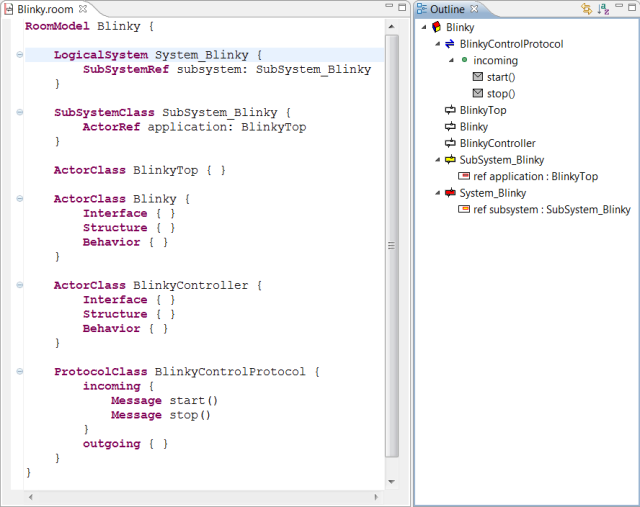
\includegraphics[width=0.8\textwidth]{images/020-Blinky03.png}
% !images/020-Blinky03.png!

With Ctrl-Shift+F or selecting \textit{Format} from the context menu you can format the text. Note that 
all elements are displayed in the outline view.

\section{Import the Timing Service}

Switching on and off the LED is timing controlled. The timing service is provided from the model library 
and must be imported before it can be used from the model.

This is the first time you use an element from the modellib. Make sure that your Java Build Path has the 
appropriate entry to the modellib. Otherwise the jave code, which will be generated from the modellib, can 
not be referenced.
(right click to \textit{Blinky} and select properties. Select the \textit{Java Build Path} tab) 
  
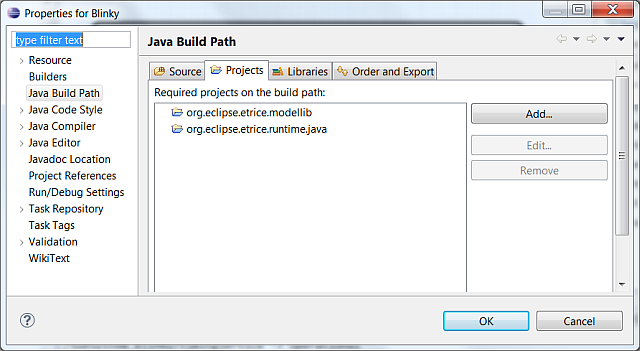
\includegraphics[width=0.8\textwidth]{images/020-Blinky16.png}
% !images/020-Blinky16.png! 

After the build path is set up return to the model and navigate the cursor at the beginning of the model 
and import the timing service: 

\begin{small}
\begin{verbatim}
RoomModel Blinky {
    
    import room.basic.service.timing.* from 
		"../../org.eclipse.etrice.modellib/models/TimingService.room" 
    
    LogicalSystem System_Blinky {
        SubSystemRef subsystem: SubSystem\_Blinky
    }
}
...     
\end{verbatim}
\end{small}

Make sure that the path fits to your folder structure. The original tutorial code is different due to the 
folder structure.  

Now it can be used within the model. Right click to \textbf{SubSystem\_Blinky} within the outline view. 
Select \textit{Edit Structure}. The \textit{application} is already referenced in the subsystem. Drag and 
Drop an \textit{ActorRef} to the \textbf{SubSystem\_Blinky} and name it \textit{timingService}. From the 
actor class drop down list select \textit{room.basic.service.timing.ATimingService}. Draw a 
\textit{LayerConnection} from \textit{application} to each service provision point (SPP) of the 
\textit{timingService}. The resulting structure should look like this:

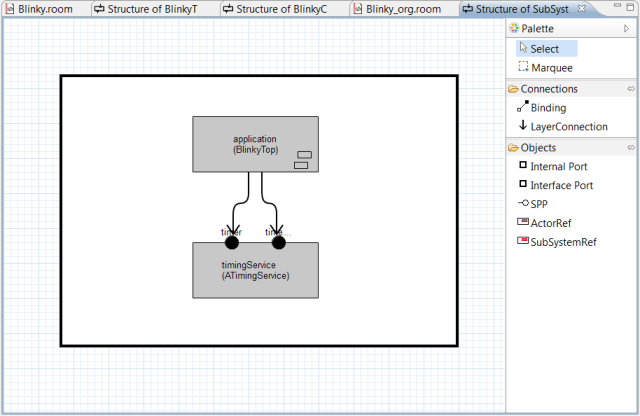
\includegraphics[width=0.8\textwidth]{images/020-Blinky06.png}
% !images/020-Blinky06.png! 

The current version of \eTrice{} does not provide a graphical element for a service access point (SAP). 
Therefore the SAPs to access the timing service must be added in the .room file. Open the 
\textit{Blinky.room} file and navigate to the \textit{Blinky} actor. Add the following line to the 
structure of the actor:

\begin{verbatim}SAP timer: room.basic.service.timing.PTimeout \end{verbatim}

Do the same thing for \textit{BlinkyController}.

The resulting code should look like this:

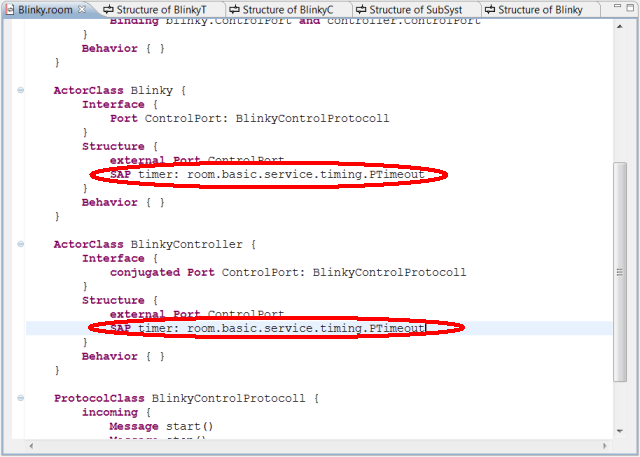
\includegraphics[width=0.8\textwidth]{images/020-Blinky07.png}
% !images/020-Blinky07.png!


\section{Finish the model structure}

From the outline view right click to \textit{Blinky} and select \textit{Edit Structure}. Drag and Drop an 
\textit{Interface Port} to the boarder of the \textit{Blinky} actor. Note that an interface port is not 
possible inside the actor. Name the port \textit{ControlPort} and select \textit{BlinkyControlProtocol} 
from the drop down list. Uncheck \textit{Conjugated} and \textit{Is Relay Port}. Click \textit{ok}. The 
resulting structure should look like this:

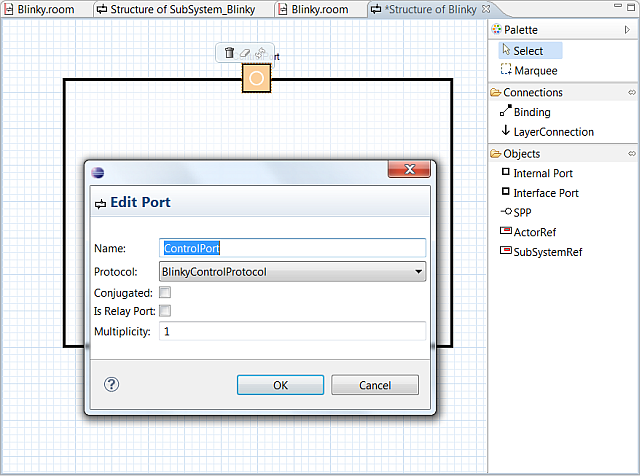
\includegraphics[width=0.8\textwidth]{images/020-Blinky04.png}
% !images/020-Blinky04.png!

Repeat the above steps for the \textit{BlinkyController}. Make the port \textit{Conjugated}

Keep in mind that the protocol defines \textit{start} and \textit{stop} as incoming messages. 
\textit{Blinky} receives this messages and therefore \textit{Blinky}'s \textit{ControlPort} must be a 
regular port and \textit{BlinkyController}'s \textit{ControlPort} must be a conjugated port.


From the outline view right click \textit{BlinkyTop} and select \textit{Edit Structure}.

Drag and Drop an \textit{ActorRef} inside the \textit{BlinkyTop} actor. Name it \textit{blinky}. From the 
actor class drop down list select \textit{Blinky}. Do the same for \textit{controller}. Connect the ports 
via the binding tool. The resulting structure should look like this:

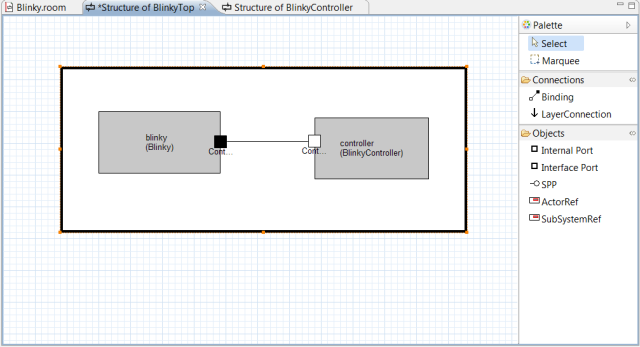
\includegraphics[width=0.8\textwidth]{images/020-Blinky05.png}
% !images/020-Blinky05.png!

\section{Implement the Behavior}

The application should switch on and off the LED for 5 seconds in a 1 second interval, then stop blinking 
for 5 seconds and start again. To implement this behavior we will implement two FSMs. One for the 1 second 
interval and one for the 5 second interval. The 1 second blinking should be implemented in 
\textit{Blinky}. The 5 second interval should be implemented in \textit{BlinkyController}. First implement 
the Controller.

Right click to \textit{BlinkyController} and select \textit{Edit Behavior}.
Drag and Drop the \textit{Initial Point} and two \textit{States} into the top state. Name the states 
\textit{on} and \textit{off}. 
Use the \textit{Transition} tool to draw transitions from \textit{init} to \textit{on} from \textit{on} to 
\textit{off} and from \textit{off} to \textit{on}.

Open the transition dialog by double click the arrow to specify the trigger event and the action code of 
each transition. Note that the initial transition does not have a trigger event.

The transition dialog should look like this:

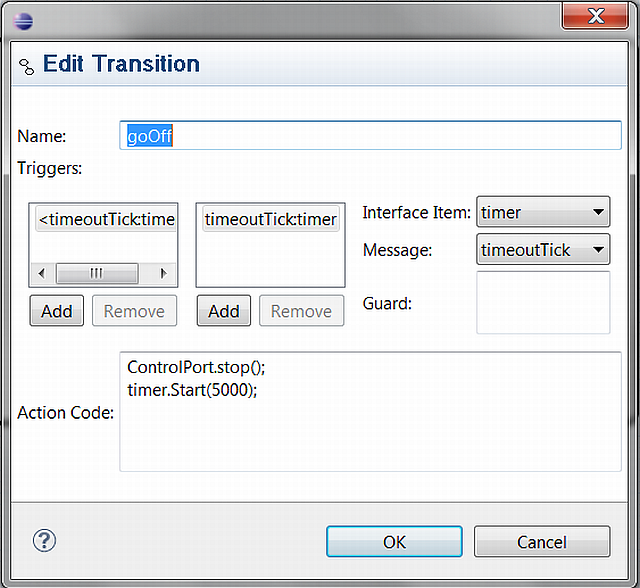
\includegraphics[width=0.8\textwidth]{images/020-Blinky09.png}
% !{width=500px}images/020-Blinky09.png! 

The defined ports will be generated as a member attribute of the actor class from type of the attached 
protocol. So, to send e message you must state \textit{port.message(param);}. In this example 
\textit{ControlPort.start()} sends the \textit{start} message via the \textit{ControlPort} to the outside 
world. Assuming that \textit{Blinky} is connected to this port, the message will start the one second 
blinking FSM. It is the same thing with the \textit{timer}. The SAP is also a port and follows the same 
rules. So it is clear that \textit{timer.Start(5000);} will send the \textit{Start} message to the timing 
service. The timing service will send a \textit{timeoutTick} message back after 5000ms.

Within each transition the timer will be restarted and the appropriate message will be sent via the 
\textit{ControlPort}. 

The resulting state machine should look like this:
(Note that the arrows peak changes if the transition contains action code.)

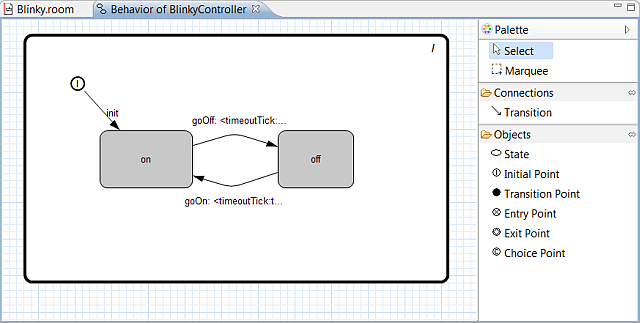
\includegraphics[width=0.8\textwidth]{images/020-Blinky10.png}
% !images/020-Blinky10.png!

Save the diagram and inspect the \textit{Blinky.room} file. The \textit{BlinkyController} should look like 
this:

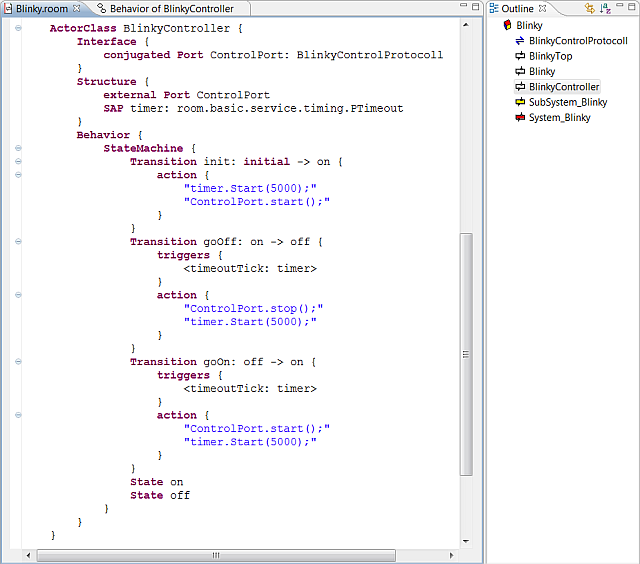
\includegraphics[width=0.8\textwidth]{images/020-Blinky11.png}
% !images/020-Blinky11.png! 
 
Now we will implement \textit{Blinky}. Due to the fact that \textit{Blinky} interacts with the GUI class a 
view things must to be done in the model file.

Double click \textit{Blinky} in the outline view to navigate to \textit{Blinky} within the model file.
Add the following code:
(type it or simply copy it from the tutorial project)

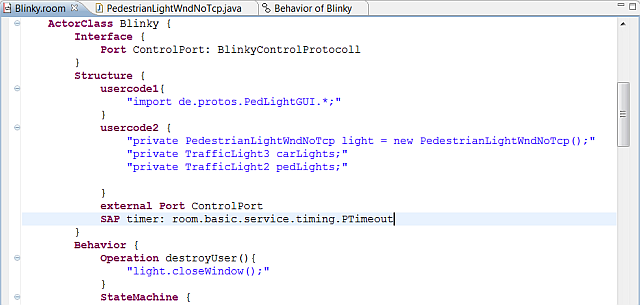
\includegraphics[width=0.8\textwidth]{images/020-Blinky12.png}
% !images/020-Blinky12.png! 

\textit{usercode1} will be generated at the beginning of the file, outside the class definition. 
\textit{usercode2} will be generated within the class definition. The code imports the GUI class and 
instantiates the window class. Attributes for the carLights and pedLights will be declared to easily 
access the lights in the state machine.
The Operation \textit{destroyUser()} is a predefined operation that will be called during shutdown of the 
application. Within this operation, cleanup of manual coded classes can be done.
 
Now design the FSM of \textit{Blinky}. Remember, as the name suggested \textit{blinking} is a state in 
which the LED must be switched on and off. We will realize that by an hierarchical FSM in which the 
\textit{blinking} state has two sub states.

Open the behavior diagram of \textit{Blinky} by right clicking the \textit{Blinky} actor in the outline 
view. Create two states named \textit{blinking} and \textit{off}. Right click to \textit{blinking} and 
create a subgraph.

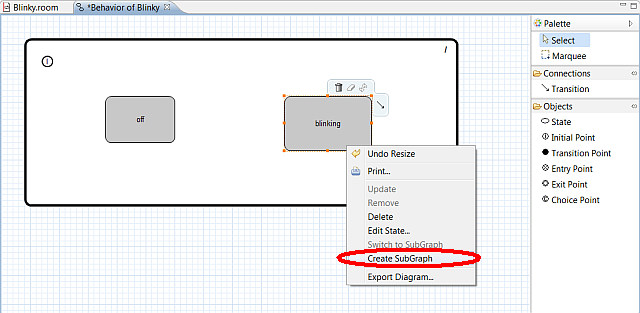
\includegraphics[width=0.8\textwidth]{images/020-Blinky13.png}
% !images/020-Blinky13.png!

Create the following state machine. The trigger events between \textit{on} and \textit{off} are the 
\textit{timeoutTick} from the \textit{timer} port. 

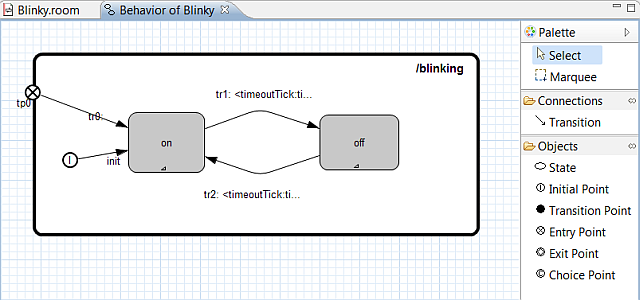
\includegraphics[width=0.8\textwidth]{images/020-Blinky14.png}
% !images/020-Blinky14.png!

Create entry code for both states by right clicking the state and select \textit{Edit State...}

Entry code of \textit{on} is:

\begin{verbatim}
timer.Start(1000);
carLights.setState(TrafficLight3.YELLOW); 
\end{verbatim}

 
Entry code  of \textit{off} is:

\begin{verbatim}
timer.Start(1000);
carLights.setState(TrafficLight3.OFF);
\end{verbatim}

Navigate to the Top level state by double clicking the \textit{/blinking} state. Create the following 
state machine:

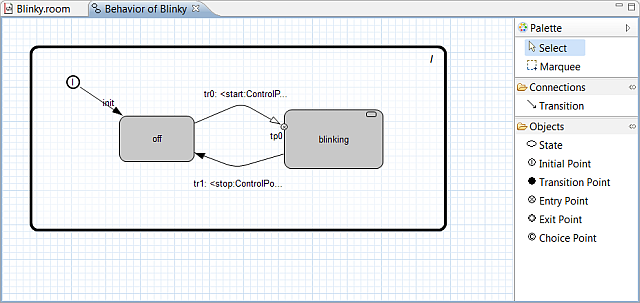
\includegraphics[width=0.8\textwidth]{images/020-Blinky15.png}
% !images/020-Blinky15.png!

The trigger event from \textit{off} to \textit{blinking} is the \textit{start} event from the 
\textit{ControlPort}.The trigger event from \textit{blinking} to \textit{off} is the \textit{stop} event 
from the \textit{ControlPort}.
Note: The transition from \textit{blinking} to \textit{off} is a so called group transition. This is a 
outgoing transition from a super state (state with sub states) without specifying the concrete leave state 
(state without sub states). An incoming transition to a super state is called history transition.   

Action code of the init transition is:

\begin{verbatim}
carLights = light.getCarLights();
pedLights = light.getPedLights();
carLights.setState(TrafficLight3.OFF);
pedLights.setState(TrafficLight2.OFF);
\end{verbatim}

Action code from \textit{blinking} to \textit{off} is:

\begin{verbatim}
timer.Kill();
carLights.setState(TrafficLight3.OFF); 
\end{verbatim}

The model is complete now. You can run and debug the model as described in getting started. Have fun.

The complete model can be found in /org.eclipse.etrice.tutorials/model/Blinky.

\section{Summary}

Run the model and take a look at the generated MSCs. Inspect the generated code to understand the runtime 
model of \eTrice{}. Within this tutorial you have learned how to create a hierarchical FSM with group 
transitions and history transitions and you have used entry code. You are now familiar with the basic 
features of \eTrice{}. The further tutorials will take this knowledge as a precondition.
